
\subsection{No available hand token}

\begin{table}[h]
	\centering
	\begin{tabular}{p{2.5cm}@{\hskip 5mm}  p{5cm}@{\hskip 5mm} p{6.5cm}} 
		\toprule
		error message   & cause      & corrective action  \\ 
		\midrule
		\midrule
		Full of action token and the chessboard has no token  & If the player has all action tokens on hand, meanwhile the board is empty without any symbole token to allow action token to implement its function &  This game needs to be restart by clicking New Game button  \\
		\midrule
		Full of Replace Token and No symbol Token  & If the player has clicked their token hand, which contains three replace tokens and no symbol tokens, the game cannot be continuously played.  &  The game should be restarted by clicking the New Game button on the top left.  \\
		\bottomrule
	\end{tabular}
\end{table}

\begin{figure}[h]
	\centering
	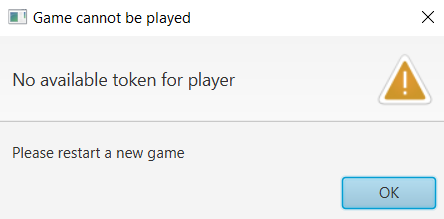
\includegraphics[width=0.6\textwidth]{image/NoToken}
	\caption{No available token hand}
	\label{fig:No available token hand}
\end{figure}